
%========= File containing the main LaTex document ========%
%                                                          %
% Copyright (C) ISI - All Rights Reserved                  %
% Proprietary                                              %
% Written by Med Hossam <med.hossam@gmail.com>, April 2016 %
%                                                          %
% @author: HEDHILI Med Houssemeddine                       %
% @linkedin: http://tn.linkedin.com/in/medhossam           %
%==========================================================%

%\documentclass[pfe]{./tpl/isipfe}
\documentclass[]{./tpl/isipfe}
\graphicspath{{./img/}}
%\usepackage{hyperref}


%=========== File containing some new commands ============%
%                                                          %
% Copyright (C) ISI - All Rights Reserved                  %
% Proprietary                                              %
% Written by Med Hossam <med.hossam@gmail.com>, April 2016 %
%                                                          %
% @author: HEDHILI Med Houssemeddine                       %
% @linkedin: http://tn.linkedin.com/in/medhossam           %
%==========================================================%

\newenvironment{changemargin}[2]{%
\begin{list}{}{%
\setlength{\leftmargin}{#1}%
\setlength{\rightmargin}{#2}%
}%
\item[]}
{\end{list}}

\makeatletter

%================= front cover variables =================%

\newcommand{\secondAuthor}[1]{\gdef\@secondAuthor{#1}}%
\newcommand{\@secondAuthor}{\@latex@warning@no@line{No \noexpand\secondAuthor given}}

\newcommand{\diplomaName}[1]{\gdef\@diplomaName{#1}}%
\newcommand{\@diplomaName}{\@latex@warning@no@line{No \noexpand\diplomaName given}}

\newcommand{\speciality}[1]{\gdef\@speciality{#1}}%
\newcommand{\@speciality}{\@latex@warning@no@line{No \noexpand\speciality given}}

\newcommand{\proFramerName}[1]{\gdef\@proFramerName{#1}}%
\newcommand{\@proFramerName}{\@latex@warning@no@line{No \noexpand\proFramerName given}}

\newcommand{\proFramerSpeciality}[1]{\gdef\@proFramerSpeciality{#1}}%
\newcommand{\@proFramerSpeciality}{\@latex@warning@no@line{No \noexpand\proFramerSpeciality given}}

\newcommand{\academicFramerName}[1]{\gdef\@academicFramerName{#1}}%
\newcommand{\@academicFramerName}{\@latex@warning@no@line{No \noexpand\academicFramerName given}}

\newcommand{\academicFramerSpeciality}[1]{\gdef\@academicFramerSpeciality{#1}}%
\newcommand{\@academicFramerSpeciality}{\@latex@warning@no@line{No \noexpand\academicFramerSpeciality given}}

\newcommand{\collegeYear}[1]{\gdef\@collegeYear{#1}}%
\newcommand{\@collegeYear}{\@latex@warning@no@line{No \noexpand\collegeYear given}}

\newcommand{\companyName}[1]{\gdef\@companyName{#1}}%
\newcommand{\@companyName}{\@latex@warning@no@line{No \noexpand\companyName given}}

%================== Signatures variables ==================%

\newcommand{\proSignSentence}[1]{\gdef\@proSignSentence{#1}}%
\newcommand{\@proSignSentence}{\@latex@warning@no@line{No \noexpand\proSignSentence given}}

\newcommand{\academicSignSentence}[1]{\gdef\@academicSignSentence{#1}}%
\newcommand{\@academicSignSentence}{\@latex@warning@no@line{No \noexpand\academicSignSentence given}}

%================== Backcover variables ==================%





\newcommand{\englishAbstract}[1]{\gdef\@englishAbstract{#1}}%
\newcommand{\@englishAbstract}{\@latex@warning@no@line{No \noexpand\englishAbstract given}}

\newcommand{\englishAbstractKeywords}[1]{\gdef\@englishAbstractKeywords{#1}}%
\newcommand{\@englishAbstractKeywords}{\@latex@warning@no@line{No \noexpand\englishAbstractKeywords given}}

\newcommand{\companyEmail}[1]{\gdef\@companyEmail{#1}}%
\newcommand{\@companyEmail}{\@latex@warning@no@line{No \noexpand\companyEmail given}}

\newcommand{\companyTel}[1]{\gdef\@companyTel{#1}}%
\newcommand{\@companyTel}{\@latex@warning@no@line{No \noexpand\companyTel given}}

\newcommand{\companyFax}[1]{\gdef\@companyFax{#1}}%
\newcommand{\@companyFax}{\@latex@warning@no@line{No \noexpand\companyFax given}}

\newcommand{\companyAddressFR}[1]{\gdef\@companyAddressFR{#1}}%
\newcommand{\@companyAddressFR}{\@latex@warning@no@line{No \noexpand\companyAddressFR given}}

\newcommand{\companyAddressAR}[1]{\gdef\@companyAddressAR{#1}}%
\newcommand{\@companyAddressAR}{\@latex@warning@no@line{No \noexpand\companyAddressAR given}}

%============= cmd for inserting blank page =============%
\newcommand\blankpage{%
    \null
    \thispagestyle{empty}%
    \addtocounter{page}{-1}%
    \newpage}

%================ document main language ================%
%\selectlanguage{english}

%================== required packages ===================%

\usepackage{tcolorbox}
\usepackage{afterpage}
\usepackage{array,longtable,multirow}% http://ctan.org/pkg/{array,longtable,multirow}
\usepackage{pifont}

\usepackage{pdflscape}
\usepackage{rotating}
\usepackage{wrapfig}

% @author: Stoufa
% the command `\makeindex` is mandatory to create the index file main.idx
% https://tex.stackexchange.com/questions/9913/input-index-file-not-found
\makeindex
\begin{document}

%=== File containing Global Configuration of the report ===%
%                                                          %
% Copyright (C) ISI - All Rights Reserved                  %
% Proprietary                                              %
% Written by Med Hossam <med.hossam@gmail.com>, April 2016 %
%                                                          %
% @author: HEDHILI Med Houssemeddine                       %
% @linkedin: http://tn.linkedin.com/in/medhossam           %
%==========================================================%

%=========== You MUST type your information here ==========%
% global_config.tex file is designed to configure your     %
% cover pages (main, back and black covers)                %
%==========================================================%

%============= Config new columns type ==============%
\newcolumntype{L}{>{\raggedright\arraybackslash}}
\newcolumntype{R}{>{\raggedleft\arraybackslash}}
\newcolumntype{C}{>{\centering\arraybackslash}}
\renewcommand{\labelitemi}{\ding{227}}
%==================================================%

%========= Config the cover section ==========%

\title{Orchestrating Critical Application Deployment with Minimal Downtime}

\author{Ben Hadj Nasr Mohamed}
%%% if necessary
% Set isBinomal to true and type second author name
%\setboolean{isBinomal}{true}
%\secondAuthor{Prénom NOM}

\diplomaName{Diplôme National d'Ingénieur en Sciences Appliquées et Technologiques}
\speciality{Computer Science and Engineering}

%% Encadrant professionnel
\proFramerName{Mr. Yazid Missaoui}
\proFramerSpeciality{Ingénieur R\&D}

%% Encadrant académique
\academicFramerName{Mrs. Yousra najjar}
\academicFramerSpeciality{Professor}

%% Entreprise d'accueil
\companyName{Adactim}

%% Année universitaire
\collegeYear{2023 - 2024}

%%%%%% Signatures section %%%%%%

% You can simply remove theses sentences by typing an empty string
% \proSignSentence{}

\proSignSentence{I authorize the student to submit his internship report.}

\academicSignSentence{I authorize the student to submit his internship report.}

%%% EN
\englishAbstract{The document outlines a comprehensive plan to transition from a slow and error-prone deployment process to a significantly faster and more reliable one. This is achieved by embracing a DevOps approach that leverages cloud computing, automation, and modern tools and methodologies. The new approach will automate the entire deployment lifecycle, incorporate security best practices, and utilize Scrum for structured project management.}

\englishAbstractKeywords{DevOps, Cloud Computing, Automation, CI/CD, Scrum}

%% if you want to get rid of the company address just set the boolean variable to false
% PS : it's optional
\setboolean{wantToTypeCompanyAddress}{true}

\companyEmail{https://adactim.com/home/}
\companyTel{+216 31 34 00 00}
\companyFax{+216 70 72 11 63}
\companyAddressFR{Technopark El Ghazela Tunis - Tunisia Tunis، 2088}

\frontmatter

%===== File containing the main cover of the document =====%
%                                                          %
% Copyright (C) ISI - All Rights Reserved                  %
% Proprietary                                              %
% Written by Med Hossam <med.hossam@gmail.com>, April 2016 %
%                                                          %
% @author: HEDHILI Med Houssemeddine                       %
% @linkedin: http://tn.linkedin.com/in/medhossam           %
%==========================================================%

%== It's advised to not modify the content of this file ===%
% To set your information, go to global_config.tex file    %
%==========================================================%

\thispagestyle{cover}%
\newgeometry{bottom=25mm,left=20mm,top=15mm,right=20mm}
\hspace{-47pt}
\begin{minipage}[l]{0.2\columnwidth}
\vspace{6mm}

\includegraphics[width=1.1\columnwidth]{LogoISI}\\
\end{minipage}
\hfill
\begin{minipage}[l]{0.6\columnwidth}
\centering
\footnotesize
\textbf{{République Tunisienne}}\\
\vspace{1.5mm}
\textbf{{Ministère de l'Enseignement Supérieur\\
et de la Recherche Scientifique}}\\
\vspace{1.5mm}
\textbf{{Université de Tunis El Manar}}\\
\vspace{1.5mm}
\textbf{{Institut Supérieur d'Informatique d’El Manar}}
\end{minipage}
\hfill
\begin{minipage}[l]{0.02\columnwidth}
\end{minipage}
\hfill
\begin{minipage}[l]{0.18\columnwidth}
\vspace{6mm}

\includegraphics[width=0.9\columnwidth]{Logo_UTM}\\
\end{minipage}
\vskip1.5cm

\begin{center}
{\LARGE{\textbf{\textsc{Rapport de Projet de Fin d'\'Etudes}}}}\\
\vskip0.5cm
\large

{\textbf{Présenté en vue de l'obtention du}}\\
\vskip2mm
{\textbf{\@diplomaName}}\\
{\textbf{Spécialité : \@speciality}}\\
{}
\end{center}

\begin{center}
\textrm{Par}\\
\vskip0.3cm
{\ifthenelse{\boolean{isBinomal}}
    {% IF TRUE
        \begin{center}
            \large\textbf{\@author}~~~~~ et ~~~~~
            \large\textbf{\@secondAuthor}
        \end{center}
    }
    {\Large\textbf{\@author}}% FALSE
}
\vskip12mm

\definecolor{isiBlue}{RGB}{31, 78, 121}

\begin{changemargin}{-9mm}{0cm}
\begin{minipage}[l]{1.1\columnwidth}
\begin{tcolorbox}[colframe=isiBlue,colback=white,boxrule=0pt,toprule=3pt,bottomrule=3pt,arc=0pt,top=0mm,right=0mm,left=0mm,bottom=0mm,boxsep=0.5mm]{
    \begin{tcolorbox}[colframe=isiBlue,colback=white, boxrule=0pt,toprule=1pt,bottomrule=1pt,arc=0pt,enlarge bottom by=-0.9mm, auto outer arc]
        \centering
        {\huge\textbf{\@title}}
    \end{tcolorbox}
}
\end{tcolorbox}
\end{minipage}
\end{changemargin}

\end{center}
\vskip8mm%

\begin{center}
\large
\begin{minipage}[c]{0.28\columnwidth}
Encadrant professionnel:\\
Encadrant académique:
\end{minipage}
\hfill
\begin{minipage}[c]{0.42\columnwidth}
\textbf{\@proFramerName}\\
\textbf{\@academicFramerName}
\end{minipage}
\hfill
\begin{minipage}[c]{0.26\columnwidth}
\@proFramerSpeciality\\
\@academicFramerSpeciality
\end{minipage}
\end{center}
\vskip16mm

\begin{center}
\large
Réalisé au sein de \@companyName\\
\vskip0.4cm
\begin{figure}[h]
\centering
{\color{isiBlue}{\fboxrule=2.5pt\fbox{
\includegraphics[width=0.4\columnwidth]{Logo_Entreprise}}}}
\end{figure}
\end{center}

\afterpage{\blankpage}

%===== File containing the black cover of the document ====%
%                                                          %
% Copyright (C) ISI - All Rights Reserved                  %
% Proprietary                                              %
% Written by Med Hossam <med.hossam@gmail.com>, April 2016 %
%                                                          %
% @author: HEDHILI Med Houssemeddine                       %
% @linkedin: http://tn.linkedin.com/in/medhossam           %
%==========================================================%

%== It's advised to not modify the content of this file ===%
% To set your information, go to global_config.tex file    %
%==========================================================%

\thispagestyle{cover}%
\hspace{-47pt}
\begin{minipage}[l]{0.2\columnwidth}
\vspace{6mm}

\includegraphics[width=1.1\columnwidth]{Logo_ISI_Black}\\
\end{minipage}
\hfill
\begin{minipage}[l]{0.6\columnwidth}
\centering
\footnotesize
\textbf{{République Tunisienne}}\\
\vspace{1.5mm}
\textbf{{Ministère de l'Enseignement Supérieur\\
et de la Recherche Scientifique}}\\
\vspace{1.5mm}
\textbf{{Université de Tunis El Manar}}\\
\vspace{1.5mm}
\textbf{{Institut Supérieur d'Informatique d’El Manar}}
\end{minipage}
\hfill
\begin{minipage}[l]{0.02\columnwidth}
\end{minipage}
\hfill
\begin{minipage}[l]{0.18\columnwidth}
\vspace{6mm}

\includegraphics[width=0.9\columnwidth]{Logo_UTM_Black}\\
\end{minipage}
\vskip1.5cm

\begin{center}
{\LARGE{\textbf{\textsc{Rapport de Projet de Fin d'\'Etudes}}}}\\
\vskip0.5cm
\large

{\textbf{Présenté en vue de l'obtention du}}\\
\vskip2mm
{\textbf{\@diplomaName}}\\
{\textbf{Spécialité : \@speciality}}\\
{}
\end{center}

\begin{center}
\textrm{Par}\\
\vskip0.3cm
{\ifthenelse{\boolean{isBinomal}}
    {% IF TRUE
        \begin{center}
            \large\textbf{\@author}~~~~~ et ~~~~~
            \large\textbf{\@secondAuthor}
        \end{center}
    }
    {\Large\textbf{\@author}}% FALSE
}
\vskip12mm

\begin{changemargin}{-9mm}{0cm}
\begin{minipage}[l]{1.1\columnwidth}
\begin{tcolorbox}[colback=white,boxrule=0pt,toprule=3pt,bottomrule=3pt,arc=0pt,top=0mm,right=0mm,left=0mm,bottom=0mm,boxsep=0.5mm]{
    \begin{tcolorbox}[colback=white, boxrule=0pt,toprule=1pt,bottomrule=1pt,arc=0pt,enlarge bottom by=-0.9mm, auto outer arc]
        \centering
        {\huge\textbf{\@title}}
    \end{tcolorbox}
}
\end{tcolorbox}
\end{minipage}
\end{changemargin}

\end{center}
\vskip8mm%

\begin{center}
\large
\begin{minipage}[c]{0.28\columnwidth}
Encadrant professionnel:\\
Encadrant académique:
\end{minipage}
\hfill
\begin{minipage}[c]{0.42\columnwidth}
\textbf{\@proFramerName}\\
\textbf{\@academicFramerName}
\end{minipage}
\hfill
\begin{minipage}[c]{0.26\columnwidth}
\@proFramerSpeciality\\
\@academicFramerSpeciality
\end{minipage}
\end{center}
\vskip16mm

\begin{center}
\large
Réalisé au sein de \@companyName\\
\vskip0.4cm
\begin{figure}[h]
\centering
{{\fboxrule=2.5pt\fbox{
\includegraphics[width=0.4\columnwidth]{Logo_Entreprise_Black}}}}
\end{figure}
\end{center}

\restoregeometry
\thispagestyle{empty}

\begin{center}
    \begin{minipage}[l]{1\columnwidth}
        \begin{tcolorbox}[colback=white,boxrule=5pt,arc=10pt,height=105mm]{
            \vspace{2cm}
            \large \@proSignSentence
            \vspace{1mm}
            \begin{center}
                \Large
                Professional Supervisor, \textbf{\@proFramerName}
            \end{center}
            \vspace{5mm}
            \hspace{0.84\columnwidth}\textbf{\large Signature}
        }
        \end{tcolorbox}
    \end{minipage}
    
    \vspace{2cm}
    
    \begin{minipage}[l]{1\columnwidth}
        \begin{tcolorbox}[colback=white,boxrule=5pt,arc=10pt,height=105mm]{
            \vspace{2cm}
            \large \@academicSignSentence
            \vspace{1mm}
            \begin{center}
                \Large
                Academic Supervisor, \textbf{\@academicFramerName}
            \end{center}
            \vspace{5mm}
            \hspace{0.84\columnwidth}\textbf{\large Signature}
        }
        \end{tcolorbox}
    \end{minipage}
\end{center}

\setcounter{page}{1}
\chapter*{\Huge Dédicaces}

\begingroup
    \large \raggedright Je dédie ce travail à :
    \vspace{4mm}
    
    Monsieur \textbf{\@proFramerName}, Monsieur \textbf{\@academicFramerName} pour m'avoir encadré et fait de leurs mieux afin de m'aider.
    
    \vspace{4mm}
    etc.
\endgroup

\vspace{8mm}
\begin{flushright}
    \LARGE \@author
\end{flushright}
\thispagestyle{frontmatter}
\chapter*{\huge Remerciements}

\begin{center}
\it \Large
    Je remercie
    
    Je suis reconnaissant
    
    J'exprime ma gratitude
\end{center}
\thispagestyle{frontmatter}

\setcounter{secnumdepth}{3}
\setcounter{tocdepth}{2}
\dominitoc
\tableofcontents
\adjustmtc
\thispagestyle{frontmatter}

\listoffigures
\thispagestyle{frontmatter}
\listoftables
\thispagestyle{frontmatter}

\chapter*{Liste des abréviations}

%=============== Glossary example ==============%
% it's an enhanced itemize list to make it      %
% sortable automatically.                       %
%===============================================%

\begin{acronyms}
    
    \sortitem[GLSI]{
        \textbf{G}énie \textbf{L}ogiciel et \textbf{S}ystèmes d’\textbf{I}nformation
    }
    
    \sortitem[GTR]{
        Génie des Télécommunications et Réseaux
    }
    
    \sortitem[GISI]{
        Génie Informatique des Systèmes Industriels
    }
    
\end{acronyms}
\thispagestyle{frontmatter}

\mainmatter
\chapter*{General Introduction}
\addcontentsline{toc}{chapter}{General Introduction}
\markboth{General Introduction}{}
\noindent In the fast-paced world of web development, users expect applications and websites to be constantly available and up-to-date. This creates a crucial challenge: how to implement new features, fix bugs, and improve performance without disrupting the user experience.
\par
\noindent Furthermore, to guarantee an impeccable user experience, testing is a vital step in the development process. However, this testing needs to be streamlined to avoid slowing down development.
\par
\noindent This need for efficiency necessitates an automated deployment process. For cloud-hosted websites, setting up such a process presents its own challenges, such as connecting various cloud services and development tools. However, it also offers unique opportunities, like streamlining the creation of the cloud infrastructure itself.
\par 
\noindent ADACTIM, a cloud and outsourcing services company whose introduction can be found in the \textbf{first chapter}, aims to establish an optimized deployment and testing process for a critical cloud-hosted web application. This will accelerate development and allow developers to focus on core coding rather than deployment tasks.
\par 
\noindent The technical development will follow the DevOps process, requiring an understanding of cloud computing and DevOps practices that will be detailed in the \textbf{second chapter}.
\par
\noindent After that we will explore the thought process behind selecting the process components in the \textbf{third chapter}.
\par 
\noindent The realiasation of the project is detailed in the last three chapters. First in the \textbf{fourth chapter}, we'll establish a solid foundation for our cloud environment using Infrastructure as Code (IaC). This involves creating scripts that automate the provisioning of cloud resources. These scripts ensure our infrastructure is not only built efficiently but also remains reusable and maintainable for future changes.
\par
\noindent Next in the \textbf{fifth chapter}, we'll implement the (CI/CD) pipeline. This pipeline acts like an automated assembly line, taking code changes and automatically triggering builds, tests, and potentially even deployments. all while establishing a DevOps workflow will bridge the gap between development and operations teams, fostering collaboration and a smoother development process.
\par
\noindent Finally in the \textbf{sixth chapter}, we'll focus on creating deployment scripts and the pipeline flow that guarantees minimal downtime during updates to the live application.
\clearpage

\chapter{General framework of the project}
\section*{Introduction}
In this chapter we will present a global overview of the project, starting with the presentation of the host organization, followed by the problematic that was the reason behind the project, and finally we will into the methodology that was adopted to achieve this project objectives.
\section{The Host Organization}
\paragraph[short]{ADACTIM}
helps businesses leverage technology to improve their operations. They specialize in cloud computing, application integration and management, enterprise resource planning (ERP), and business intelligence (BI).  They operate internationally across Europe, North Africa, and Africa.

\begin{figure}[htpb]
    \centering
    \frame{
\includegraphics[width=0.5\columnwidth]{logo-adactim.png}}
    \caption{Logo Entreprise Adactim}
    \label{fig:logo_Adactim}
\end{figure}

\subsection*{ \textbullet\ Adactim  Mission}
ADACTIM can enable a company to benefit from technological transformations in the areas of IT infrastructure and integrated business systems allowing it to focus its energy on its core business.
\\
\emph{"Their mission is to facilitate businesses' access to technological innovations, to simplify their daily use, allowing the company to be more efficient and competitive.
With this, the client company can focus its resources on its development and its customers. the company will be well-equipped with business software and IT infrastructure and outsource appropriate operations processes."}
\section{Problematic}

\subsection{Existing study}
\noindent
\textbf{Description of the Current Environment:}
\\
Some applications that are managed by ADACTIM currently runs on a manually provisioned Azure cloud infrastructure managed through the web portal. Which means the actions to these infrastructures are done through a graphical interface provided by azure.
\\
\textbf{Analysis of Existing Deployment Processes:}

\begin{figure}[htpb]
    \centering
    \frame{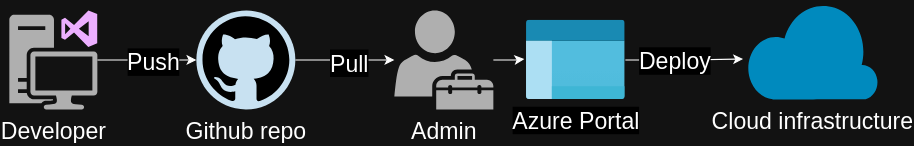
\includegraphics[width=0.8\columnwidth]{existing_stratigy.png}}
    \caption{existing strategy of the application deployment}
    \label{fig:existing_strategy}
\end{figure}

The deployment of applications in our current setup involves several steps, including code preparation, testing, deployment scheduling, and monitoring. Each deployment requires coordination between multiple teams, including developers, quality assurance, and system administrators.
Strengths and Weaknesses of the Current Approach:
\\
\textbf{Strengths:}
\begin{itemize}
    \item Our current deployment process follows a structured workflow, ensuring thorough testing before releasing applications into production.
    \item Effective communication and collaborative problem-solving are facilitated by teamwork during deployments.
\end{itemize}
\textbf{Weaknesses:}
\begin{itemize}
    \item Extended outages caused by inefficient deployment practices negatively impact business continuity and revenue.
    \item Limited automation in certain areas leads to manual errors and delays during deployments.
\end{itemize}
\noindent
\subsection{Problematic:}
\par
While our current deployment process prioritizes rigorous testing and cross-team collaboration, it faces significant challenges impacting both efficiency and reliability. One critical issue lies in the protracted nature of deployment timelines. This stems from the inherent complexity of coordinating and executing numerous manual testing processes. Consequently, not only are the releases of crucial applications delayed but the potential for human error during manual interventions is also amplified
\par
In essence, our current application deployment process faces a critical challenge: balancing the strengths of its structured workflow and collaborative approach with the need for faster, more automated deployments.

\section{Proposed Deployment Optimization Solution}
In order to address the identified challenges, we propose a solution that leverages modern technologies and methodologies like Devops.
\begin{itemize}

    \item \textbf{Provisioning and Configuration Management:}
          Automate the provisioning and configuration of cloud infrastructure and application environments to ensure consistency and reliability using Infrastructure as Code (IaC) and Configuration Management tools.

    \item \textbf{Automating the build and testing process:}
          minimize manual intervention and expedite development cycles by leveraging automation across the build and testing pipeline. This not only reduces human error but also frees up valuable time for developers to focus on core tasks.
    \item \textbf{implementing a Deployment strategy:}
          Implement a deployment strategy that leverages automation to ensure seamless and efficient application deployments, minimizing downtime and errors. By applying these pattern principles:
          \begin{itemize}
              \item \textbf{Rightsize resources for each environment:} ensuring that the resources allocated to each environment are appropriate for the expected load. We can do this by implementing workspaces in Terraform.
              \item \textbf{Delete non-production environments:} ensuring that non-production environments are deleted when they are no longer needed.
          \end{itemize}
\end{itemize}

\section{Methodology of the project}
While some projects might seem straightforward, a defined methodology is crucial for achieving success. This framework provides a roadmap, ensuring tasks are completed efficiently and in the right order. By following a methodology, we can avoid common pitfalls, manage our time effectively, and ultimately deliver a successful project.
\subsection*{ \textbullet\ Agile vs traditional methodologies}
\begin{longtable}[c]{
    |p{.45\textwidth}
    |p{.45\textwidth}|
    }
    \caption{the significant differences between traditional and agile project methodologies. \cite{webArticle1}}
    \label{tab:traditional_vs_agile}                                                           \\
    \hline
    \textbf{ Traditional Methodology }         & \textbf{ Agile Methodology }                  \\
    \hline
    The Waterfall model is used.               & Iterative and incremental development.        \\
    \hline
    Emphasis on planning and design.           & Emphasis on flexibility and adaptability.     \\
    \hline
    Emphasis on deliverables and completion    & Emphasis on customer satisfaction             \\
    \hline
    Projects are completed in phases.          & Projects are completed in sprints.            \\
    \hline
    The strict change management process.      & Encourages changes and improvements.          \\
    \hline
    Team roles and responsibilities are fixed. & Team roles and responsibilities are flexible. \\
    \hline
    Limited customer involvement               & High customer involvement                     \\
    \hline
    Risk management is proactive               & Risk management is reactive                   \\
    \hline
\end{longtable}
the choice between agile and traditional methodologies hinges on how much flexibility is needed. Agile thrives on an iterative approach. The team continuously works in short cycles, delivering features and gathering feedback to adapt and refine the project as it goes. This makes it ideal for DevOps, where requirements can evolve quickly. Traditional methods, on the other hand, emphasize upfront planning with a detailed roadmap. While this can be beneficial for projects with clear goals from the beginning, it can hinder DevOps teams who need to be adaptable and responsive to new information or feedback throughout the project lifecycle.
\subsection*{ \textbullet\ The Agile methodology}
\emph{"While seemingly designed for larger teams, Agile methodologies offer valuable structure even for single-person projects. Their core principles of iterative development, continuous improvement, and flexibility empower individuals to efficiently manage projects."}\cite{webArticle2}
\textbf{scrum:} Scrum is an agile framework that helps teams structure their work into short development cycles called sprints. Scrum teams commit to shipping work at the end of each sprint and adopt practices and a team structure that helps them achieve this cadence. Scrum takes the agile principles one step further, creating a structure that helps teams live the agile principles in their day-to-day work. Scrum is a well-documented agile framework that many teams can adopt without much disruption.
\subsection*{ \textbullet\ Verdict:}
Considering the project's potential for evolving requirements and the benefits of iterative development, Scrum emerges as the optimal choice. Its focus on defined sprints, adaptability, and a structured approach to project management, even for solo developers, aligns perfectly with our project needs.

\subsection*{ \textbullet\ The implementation of Scrum process}
This overview outlines how we will be implementing the Scrum process to manage our project:
\begin{itemize}
    \item \textbf{Scrum events:} \begin{itemize}
              \item \textbf{Retrospective (Weekly):} Held with the company supervisor to review the previous sprint, identify areas for improvement, and adapt the process for the upcoming sprint. This meeting can take place in person at the supervisor's office or virtually using Microsoft Teams.
              \item \textbf{Sprint Planning (Before Each Sprint):} Select items from the backlog and commit to delivering them during the upcoming sprint (a short iteration typically lasting 2 weeks).
          \end{itemize}
    \item \textbf{Scrum implementation:} \begin{itemize}
              \item \textbf{Product Backlog:} I will maintain a product backlog that outlines all the features and functionalities desired in the final product.
              \item \textbf{Sprint Planning:} Before each sprint, a sprint planning meeting is held by the supervisor and me to select a set of items from the top of the product backlog that we commit to delivering during the upcoming sprint. This selection is called the sprint backlog.
              \item \textbf{Sprint Execution:} I deliver the items in the sprint backlog. with each sprint lasting two weeks.
              \item \textbf{Sprint Retrospective:} At the end of each sprint, I will hold a sprint retrospective meeting with the company supervisor. This meeting will focus on reviewing what areas need improvement in the upcoming sprint.
          \end{itemize}
\end{itemize}

\begin{figure}[htpb]
    \centering
    \frame{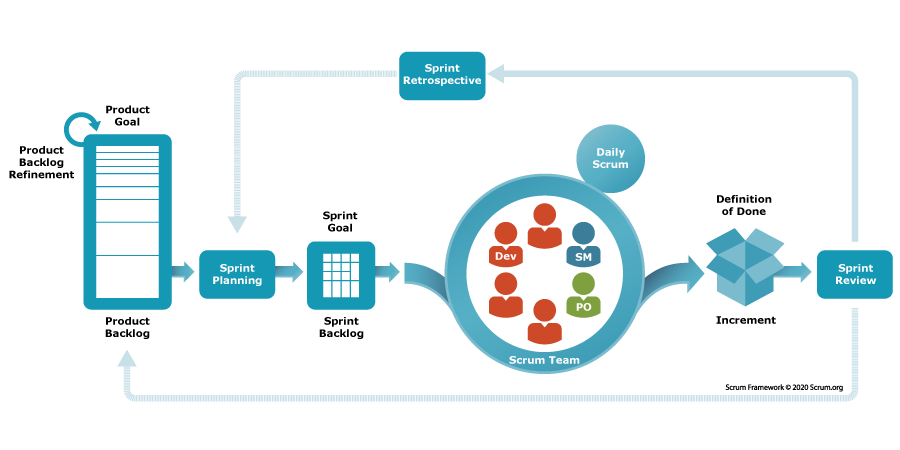
\includegraphics[width=0.8\columnwidth]{scrum-framework-9.29.23.png}}
    \caption{Scrum process \cite{webArticle2}}
    \label{fig:scrum_process}
\end{figure}

By following the Scrum process and maintaining open communication, we can ensure a successful project that delivers value iteratively while continuously adapting to feedback and changes.

\section*{Conclusion}
This chapter outlined the challenges associated with our current applications deployment process, which prioritizes thorough testing and collaboration but suffers from lengthy timelines and manual errors. To address these shortcomings, we proposed a new approach that leverages modern technologies and methodologies to achieve faster, more reliable deployments.
\par
The proposed solution emphasizes automation throughout the deployment lifecycle, encompassing infrastructure provisioning, build and testing processes, and the deployment strategy itself. This will minimize manual intervention, reduce errors, and expedite deployments. Additionally, the strategy incorporates security best practices and performance optimization techniques to ensure the applications' continued reliability and availability.
\par
Finally, we discussed the methodology Scrum that will be adopted to manage the project. This agile framework will provide a structured approach to project management.
\par
The next chapter, we will provide a comprehensive exposition to many concepts in the field of DevOps and cloud computing, which will be prove essential to understanding the project's technical aspects.
\clearpage

\chapter{Detailed Existing study}

\section*{Introduction}
In this chapter, we will explain various concepts that are crucial for the subsequent sections of this report. We will also do a thorough detailed study of the current environment the existing architecture and the deployment process.

\section{Cloud Computing}
\paragraph*{Definition:}
Cloud computing is the on-demand availability of computer system resources, especially data storage and computing power, without direct active management by the user. A simple way to describe the Cloud is its multiple data centers available to many users over the Internet.
\par
\noindent
Cloud computing services are offered by various providers, with Amazon Web Services, Microsoft Azure, and Google Cloud Platform being some of the major players in the field.
\subsection*{Comparative study between cloud providers}
So it makes sense to compare the three major cloud providers to see which one is the best for our project.
\subsubsection*{strengths of the three major cloud providers \cite{webArticle1}}
\begin{itemize}
    \item \textbf{Amazon Web Services (AWS):} AWS has had almost a 7-year head-start and vastly more offerings at present than other competitors. With that head start, the available talent pool is larger, meaning that more people know AWS.
    \item \textbf{Microsoft Azure:} Azure provides a pretty compelling transition path to the cloud, also Microsoft has a large number of enterprise customers, and many of them are already using Microsoft products. This makes it easier for them to use Azure.
    \item \textbf{Google Cloud Platform (GCP):} Google just happens to originated one of the most popular container orchestration systems, that being Kubernetes. and with that, it has been able to leverage that reputation to attract customers to its cloud platform.
\end{itemize}
\subsubsection*{Weaknesses of the three major cloud providers \cite{webArticle1}}
\begin{itemize}
    \item \textbf{Amazon Web Services (AWS):} With its vast growth Amazon (the company that owns AWS) has become a direct rival to many retailers, and that has led to some customers looking for alternatives.
    \item \textbf{Microsoft Azure:} For the past decade or so, open-source software has found great acceptance, both on-prem and in the cloud, largely due to organizations seeking alternatives to commercial software vendors like Microsoft.
    \item \textbf{Google Cloud Platform (GCP):} Google has a reputation for killing off products that don't meet its expectations, and that has led to some customers being wary of using Google Cloud Platform.
\end{itemize}
\subsection*{Verdict}
since this project is about transitioning to the cloud, and the fact that the company Adactim has a golden partnership with Microsoft, we will be using Microsoft Azure as our cloud provider.


\section{Cloud Computing Services}
\paragraph*{Definition:} Cloud computing services are a broad set of services that are delivered over the internet. These services are divided into three main categories: Infrastructure as a Service (IaaS), Platform as a Service (PaaS), and Software as a Service (SaaS).
\subsection*{IaaS}
\noindent
\textbf{Definition:} IaaS provides virtualized computing resources that require the developer to manage the infrastructure, including the network, servers, and operating systems. and with this comes great flexibility and scalability.
\noindent \\
\textbf{Offered Services:} Azure offers a wide range of IaaS services, including virtual machines, storage, and networking. With this, we can simulate the on-premises infrastructure in the cloud with minimal changes.
\subsection*{PaaS}
\noindent
\textbf{Definition:} PaaS provides a platform allowing developers to build, run, and manage applications without the complexity of building and maintaining the infrastructure. This allows developers to focus on the application itself.
\noindent \\
\textbf{Offered Services:} Some of the PaaS services offered by Azure include Azure App Service and Azure Functions. and these services have built-in deployment strategies that can be selected.
\subsection*{SaaS}
\noindent
\textbf{Definition:} SaaS is a software distribution model in which applications are hosted by a third-party provider so developers don't have to install, maintain, or update the software.
\noindent \\
\textbf{Offered Services:} Azure offers a wide range of SaaS services, including Office 365, Dynamics 365, and many more. Unfortunately, these services are not relevant to us since we cannot use them to host our application.
\subsection*{Verdict}
After this brief overview of the cloud computing services, we can conclude that the IaaS and PaaS services are the most relevant to us, so I will implement the deployment plan using both of them and choose the most suitable one.
\section{Infrastructure Study}
The company is currently using the baseline web application architecture provided by Microsoft\cite{webArticle6}.
This figure \ref{fig:gloabal_architecture} presents the global architecture of the application.

\begin{figure}[htpb]
    \centering
    \frame{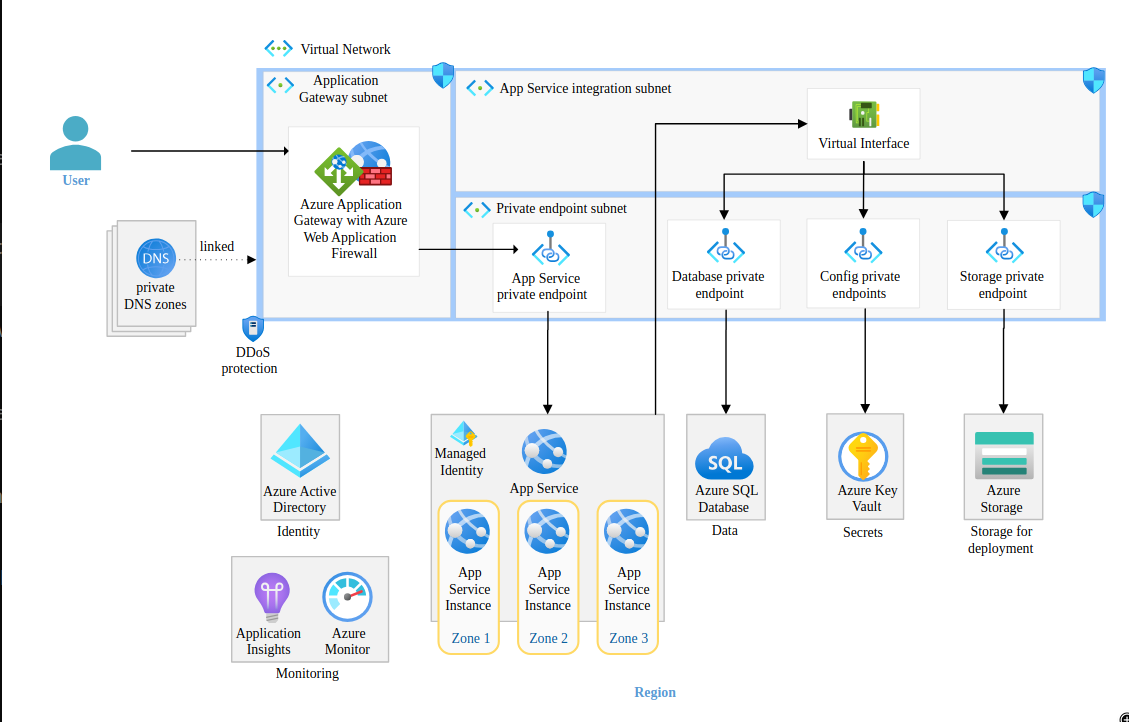
\includegraphics[width=0.5\columnwidth]{global_architecture.png}}
    \caption{gloabal architecture}
    \label{fig:gloabal_architecture}
\end{figure}

\noindent \textbf{Description:} The architecture exposes a public endpoint via Azure Application Gateway with a Web Application Firewall. The App Service application uses virtual network integration to securely communicate to Azure PaaS services such as Azure Key Vault and Azure SQL Database.

\subsection*{Componants of the architecture}
\begin{itemize}
    \item \textbf{Virtual Network:} This is the fundamental building block for your private network in Azure. It provides isolation and protection for your resources.
    \item \textbf{App Service:} This service is used to host the web application. It provides a fully managed platform for building, deploying, and scaling web apps.
    \item \textbf{Azure SQL Database:} This service is used to store the application data. It provides a fully managed relational database with built-in high availability and security.
    \item \textbf{Azure Key Vault:} This service is used to store and manage application secrets. It provides a secure and centralized storage for application secrets.
    \item \textbf{Azure Application Gateway:} This service is used to protect the web application from common web vulnerabilities. It provides a web application firewall and other security features.
    \item \textbf{Azure Monitor:} This service is used to monitor the health of the web application. It provides logging and application telemetry to monitor the health of the application.
    \item \textbf{Azure DevOps:} This service is used to automate the deployment of the web application. It provides a set of tools for building, testing, and deploying applications.
    \item \textbf{Virtual Interface:} This service is used to connect the web application to the virtual network. It provides a secure and private connection to the web application.
    \item \textbf{Application Insights:} This service is used to monitor the performance of the web application. It provides real-time monitoring and analytics for the web application.
    \item \textbf{Private DNS Service:} This service is used to resolve the DNS names of the Azure PaaS services. It provides a secure and private DNS resolution for the web application.
    \item \textbf{Private endpoint:} This service is used to connect the web application to the Azure PaaS services. It provides a secure and private connection to the Azure PaaS services.
\end{itemize}

\subsection*{Network flows}
\textbf{Inbound flow:}
\begin{itemize}
    \item The user issues a request to the Application Gateway public IP.
    \item The WAF rules are evaluated.
    \item The request is routed to an App Service instance through the private endpoint.
\end{itemize}
\textbf{App Service to Azure PaaS services flow:}
\begin{itemize}
    \item App Service makes a request to the DNS name of the required Azure service. The request could be to Azure Key Vault to get a secret, Azure SQL Database.
    \item The request is routed to the service through the private endpoint.
\end{itemize}

\textbf{Deploying to the app service:} \\
The deployment process is initiated from the Azure portal by the admin from his machine.

\subsection*{Architecture characteristics}
\begin{itemize}
    \item For security reasons, the network in this architecture has separate subnets for the Application Gateway, App Service integration components, and private endpoints. Each subnet has a network security group that limits both inbound and outbound traffic for those subnets to just what is required.
    \item The App Service baseline configures authentication and authorization for user identities (users) and workload identities (Azure resources) and implements the principle of least privilege.
    \item Azure Monitor collects and analyzes metrics and logs from your application code, infrastructure (runtime), and the platform (Azure resources).
\end{itemize}
\section{Deployment Process}
The process of releasing a new application version or update in our system follows a multi-step approach. This approach ensures a smooth transition from development to production and minimizes the risk of introducing issues.
Here's a breakdown of the key stages involved:
\begin{itemize}
    \item \textbf{Code Preparation:} During this stage, developers finalize the code for the new application version or update. This may involve tasks like code reviews, bug fixing, and integration with existing systems.
    \item \textbf{Testing:} Once the code is prepared, it undergoes rigorous testing by the Quality Assurance (QA) team. This testing verifies that the application functions as intended identifies and resolves any bugs or errors, and ensures compatibility with different environments.
    \item \textbf{Deployment Scheduling:} Following successful testing, a deployment plan is created. This plan defines the specific time and method for releasing the application to users. The plan often involves coordination between development, QA, and system administration teams to ensure a smooth rollout and minimal disruption to ongoing operations.
    \item \textbf{Deployment:} During deployment, the application is transferred from its development environment to the production environment where it will be used by end-users. This process may involve tasks like uploading application files, configuring settings, and integrating with databases or other systems.
    \item \textbf{Monitoring:} After deployment, the system administrators closely monitor the application's performance and functionality. This monitoring helps to identify any issues that may arise after the release and allows for prompt intervention if necessary.
\end{itemize}
Effective collaboration between development, QA, and system administration teams is crucial throughout this process. Clear communication and well-defined roles ensure a successful application deployment with minimal downtime and a positive experience for end-users.
\section{Description of available tools}
\subsection*{Terraform}

\begin{figure}[htpb]
    \centering
    \frame{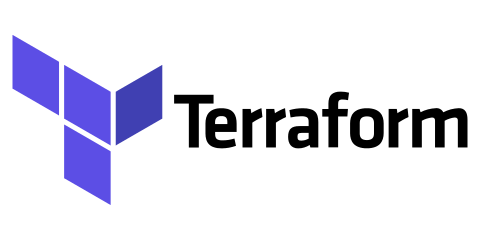
\includegraphics[width=0.5\columnwidth]{Terraform.png}}
    \caption{Terraform}
    \label{fig:terraform}
\end{figure}

\textbf{Definition:} Imagine building your software on a foundation pre-designed with specific instructions, rather than individually placing each brick. This is the essence of Terraform, an open-source IaC tool. It allows you to define the infrastructure your application needs using a simple language, similar to writing instructions. This simplifies managing resources across different environments (cloud-based or on-premises) with consistent configurations, ensuring everything is built according to your specifications.
\par
\textbf{Alternatives:}
\begin{itemize}
    \item \textbf{Azure Resource Manager (ARM) templates:} These templates are native to Azure, offering familiarity and direct management within the platform. However, they require more technical knowledge and lack the flexibility and reliability of IaC tools like Terraform.
    \item \textbf{Bicep} Think of Bicep as a specialized architect fluent in Azure, Microsoft's cloud platform. It speaks Azure's language directly, making it easier to design and manage resources within that specific environment. However, since its expertise is limited to Azure it does not have the community support offered by an open-source project like Terraform.
\end{itemize}
By understanding these factors, we can make the informed decision that the IaC tool that best suits our requirements is Terraform.
\subsection*{Azure DevOps}

\begin{figure}[htpb]
    \centering
    \frame{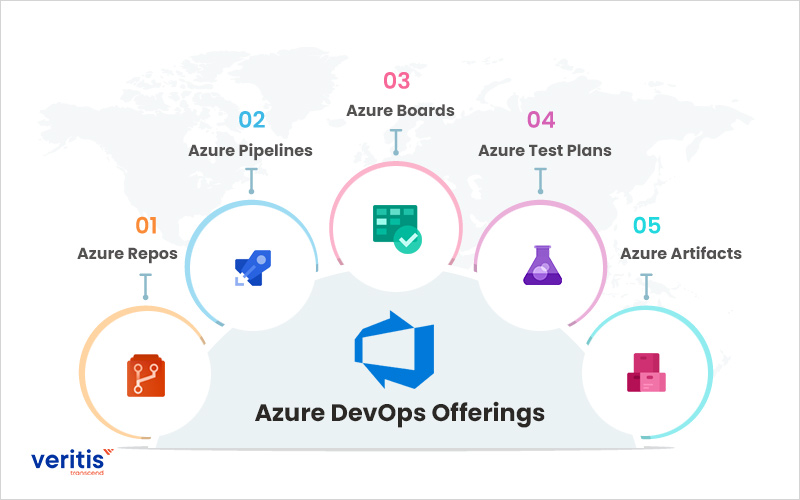
\includegraphics[width=0.5\columnwidth]{azure-devops-offerings.jpg}}
    \caption{Azure DevOps}
    \label{fig:Azure_DevOps}
\end{figure}

\textbf{Definition:} This platform acts as a comprehensive toolkit for software teams, offering various features to manage the entire development lifecycle efficiently.
\par
\textbf{Features:}
\begin{itemize}
    \item \textbf{Azure Repos:} This feature keeps your code organized and secure, just like a well-structured library holding all your project versions. It can use either Git or Team Foundation Version Control (TFVC) to manage your code.
    \item \textbf{Azure Pipelines:}  This service automates tasks like compiling code, running tests, and deploying new versions, saving time and minimizing errors.
    \item \textbf{Azure Boards:} Planning and tracking progress becomes transparent with this feature. It provides Kanban boards visually displaying tasks, backlogs listing upcoming work, and sprint planning tools.
    \item \textbf{Azure Artifacts:} Sharing reusable components becomes effortless with this feature. Think of it as a shared storage space for code modules, containerized applications, and other resources your team can easily access and reuse across projects.
\end{itemize}
\section{Overview of the scrum process}
This overview outlines how we will be implementing the Scrum process to manage our project:
\begin{itemize}
    \item \textbf{Scrum events:} \begin{itemize}
              \item \textbf{Retrospective (Weekly):} Held with the company supervisor to review the previous sprint, identify areas for improvement, and adapt the process for the upcoming sprint. This meeting can take place in person at the supervisor's office or virtually using Microsoft Teams.
              \item \textbf{Sprint Planning (Before Each Sprint):} Select items from the backlog and commit to delivering them during the upcoming sprint (a short iteration typically lasting 2 weeks).
          \end{itemize}
    \item \textbf{Scrum implementation:} \begin{itemize}
              \item \textbf{Product Backlog:} I will maintain a product backlog that outlines all the features and functionalities desired in the final product.
              \item \textbf{Sprint Planning:} Before each sprint, a sprint planning meeting is held by the supervisor and me to select a set of items from the top of the product backlog that we commit to delivering during the upcoming sprint. This selection is called the sprint backlog.
              \item \textbf{Sprint Execution:} I deliver the items in the sprint backlog.
              \item \textbf{Sprint Retrospective:} At the end of each sprint, I will hold a sprint retrospective meeting with the company supervisor. This meeting will focus on reviewing what areas need improvement in the upcoming sprint.
          \end{itemize}

\begin{figure}[htpb]
    \centering
    \frame{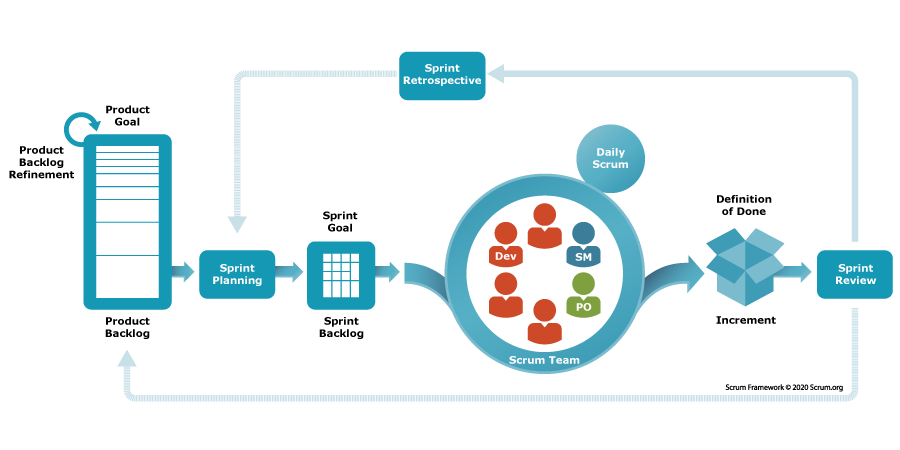
\includegraphics[width=0.8\columnwidth]{scrum-framework-9.29.23.png}}
    \caption{Scrum process  }
    \label{fig:scrum_process}
\end{figure}

\end{itemize}
By following the Scrum process and maintaining open communication, we can ensure a successful project that delivers value iteratively while continuously adapting to feedback and changes.
\section*{Conclusion}
This chapter has comprehensively analyzed the current state of our cloud environment, infrastructure, and deployment process. We compared various cloud service models, ultimately selecting Microsoft Azure due to its alignment with our company's existing partnership and strategic goals. Within Azure, we identified Infrastructure as a Service (IaaS) and Platform as a Service (PaaS) as the most suitable offerings for our application's needs.
\par
Our in-depth examination of the existing infrastructure revealed a secure and well-structured architecture leveraging Azure's robust security features. Moving forward, we will delve deeper into Terraform and Azure DevOps, exploring their functionalities for enhanced infrastructure management and automated deployment processes. This comprehensive analysis establishes a solid foundation for transitioning to a secure, efficient, and automated cloud-based deployment framework.
\par
To ensure an iterative and adaptable development approach, we will be implementing the Scrum process. This agile framework involves regular sprint cycles where we collaboratively define goals, execute tasks, and reflect on improvements. Through continuous feedback and adaptation within sprints, we can ensure the project delivers value efficiently while addressing evolving requirements.

\begin{figure}
    \centering
    \frame{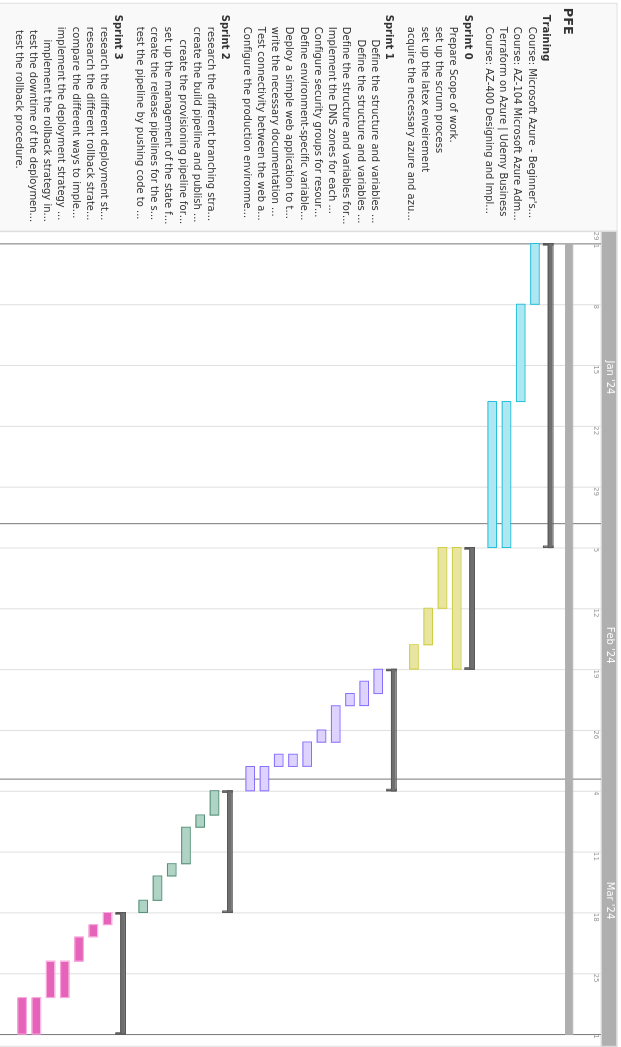
\includegraphics[width=0.84\columnwidth]{grantt.png}}
    \caption{This is the grantt chart of the scrum process} 
    \label{fig:scrum_process}
\end{figure}

\clearpage


\chapter{The provisioning of the infrastructure}

\section*{Introduction}
\noindent
The first sprint of this project focused on provisioning the necessary cloud resources and setting the connections between them. In this chapter, we will present how we customized the architecture to our needs and the challenges we faced during the process, and we will also showcase the features implemented in the terraform modules.

\section{Activities Completed}
\begin{itemize}
    \item \textbf{Azure account setup:} We created an Azure account using the student package offer.
    \item \textbf{Azure CLI installation:} We installed the Azure CLI to manage our Azure resources.
    \item \textbf{created the necessary modules:} For a better organization of our code, we separated the resources into modules: the web app module, the database module and the storage account module.
    \item \textbf{established the network configurations:} We provisioned the virtual network and the DNS zones for each module and added the necessary links.
    \item \textbf{set up the different workspaces:} We created different workspaces for each environment (dev, QA, prod) and set the default values for each environment.
    \item \textbf{tested the architecture:} We tested the architecture by deploying the provisioned resources and deploying a simple web application.
    \item \textbf{wrote the documentation:} We wrote the documentation explaining how to modify the different variables and how to use the different workspaces(I auto-generated the documentation for the modules to ensure consistency using terraform-docs).
\end{itemize}
\section{The modified architecture:}
the slight modification made to the original architecture consisted of the removal of the application gateway due to its high price so the user will just have to access the web app directly which is acceptable since we only have one web app.
\\ the new simplified architecture is shown in figure \ref{fig:new_arch}.

\begin{figure}[htpb]
    \centering
    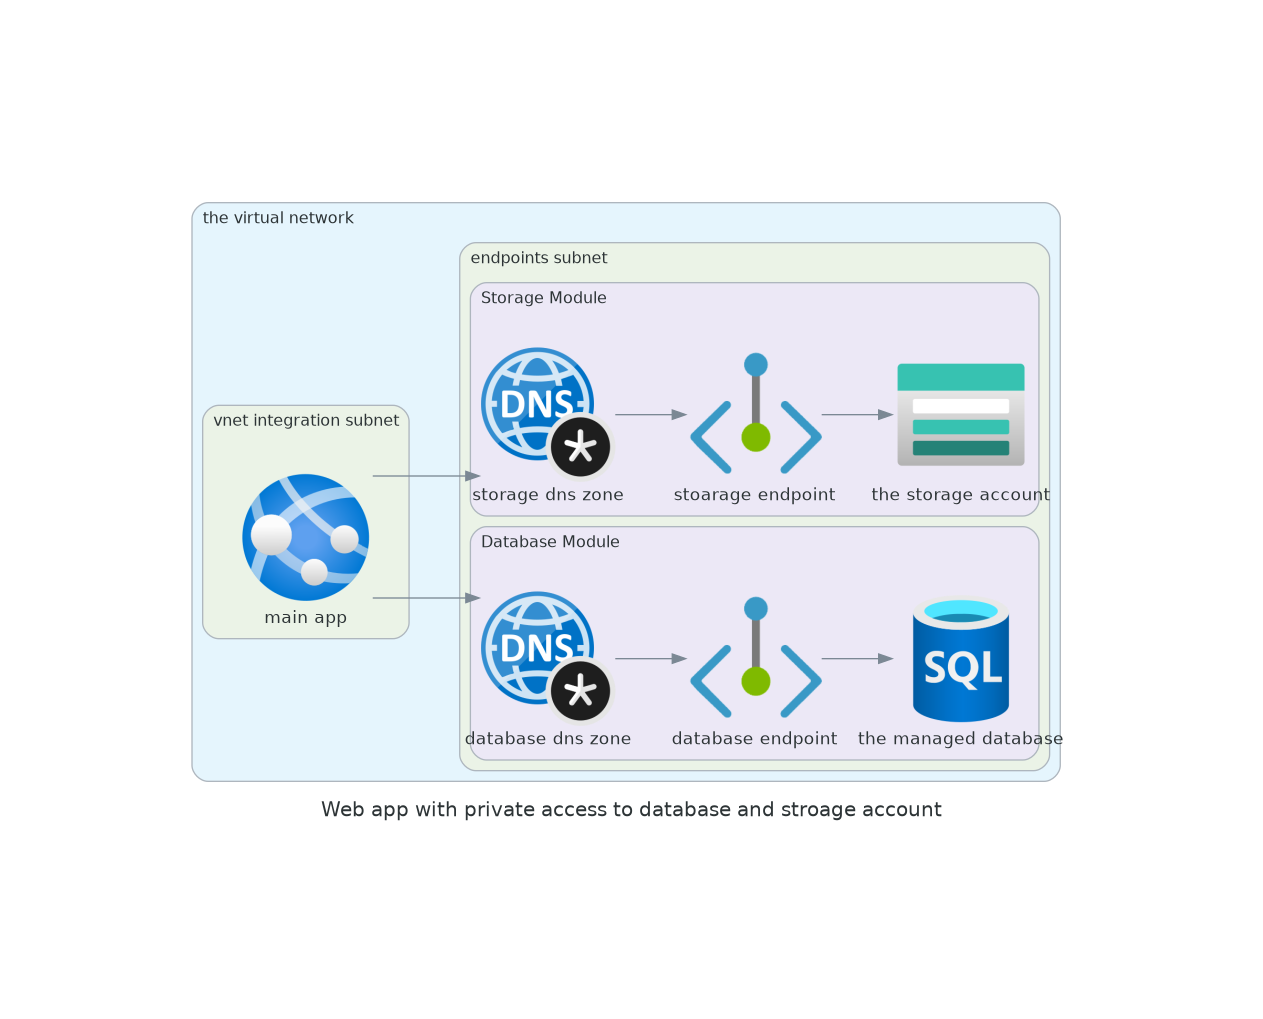
\includegraphics[width=0.8\textwidth]{web_app_with_private_access_to_database_and_stroage_account.png}
    \caption{The new architecture}
    \label{fig:new_arch}
\end{figure}

\section{Delivrables:}
the deliverables for this sprint are the terraform configuration that adapts to three different workspaces:
\begin{itemize}
    \item \textbf{dev:} the development environment:
    \begin{itemize}
        \item the resources are the most basic cost to optimize the cost.
        \item It also has a VM with a public IP inside the virtual network to access the database and the storage account.
        \item the web app and the VM can only be accessed from the CIDN given in the variables.
    \end{itemize}
    \item \textbf{QA:} the quality assurance environment:
    \begin{itemize}
        \item the resources are a bit more expensive to better simulate the production environment.
        \item It also has a VM with a public IP inside the virtual network to access the database and the storage account.
        \item it is open to the public.
    \end{itemize}
    \item \textbf{prod:} the production environment.
    \begin{itemize}
        \item the resources are the most expensive to ensure the best performance.
        \item it is open to the public.
    \end{itemize}
\end{itemize}
\subsection*{the file structure:}
this figure \ref{fig:file_structure} shows the file structure of the terraform configuration.

\begin{figure}[htpb]
    \centering
    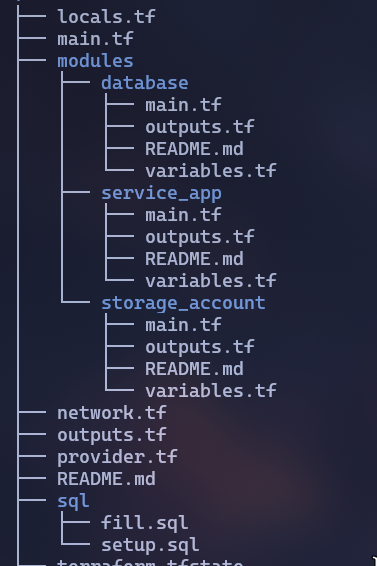
\includegraphics[width=0.3\textwidth]{file_structure.png}
    \caption{The file structure}
    \label{fig:file_structure}
\end{figure}
To promote code reusability, maintainability, and clarity, we adopted a modular approach for our Terraform configuration. This involved structuring the code into distinct modules, each encapsulating a specific aspect of the infrastructure (e.g., web app, database, storage account). This approach allows us to manage and update each module independently, and to reuse them across different environments.
\par
Furthermore, to ensure consistency and streamline configuration changes, we grouped frequently used variables like SKU names, VNet prefixes, and subnet prefixes into a dedicated local.tf file.
\par
This combined approach of modular structure and centralized variable management promotes efficient and well-organized Terraform configuration, fostering long-term project maintainability and scalability.
\section{Challenges:}
\subsection*{the problem:}
The main challenge we faced during Sprint 1 was configuring the DNS zones to enable communication between the web application and the database. Despite successfully provisioning the necessary cloud resources, the web application encountered issues resolving the hostname of the database. This meant the application couldn't locate the database to retrieve or store data, hindering core functionality. Troubleshooting involved verifying several aspects:

\begin{figure}[htpb]
    \centering
    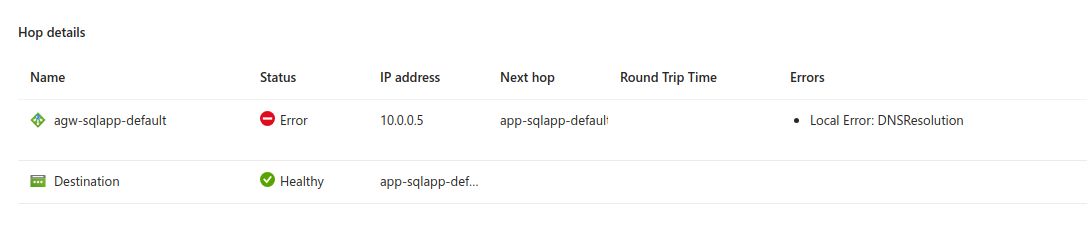
\includegraphics[width=0.8\textwidth]{connnectivity_problem.png}
    \caption{connnectivity problem}
    \label{fig:connection_problem}
\end{figure}

\begin{itemize}
    \item \textbf{DNS record configuration:} We double-checked the DNS record types (likely A record) and their values (database hostname and IP address) within the configured DNS zone. Any typos or incorrect mappings could have caused resolution issues.
    \item \textbf{Network security group (NSG) rules:} We had to verify the NSG rules to ensure the web application could communicate with the database.
    \item \textbf{verify connections:} We had to verify that the database was accessible from the web application. and that the web could access the DNS server.
\end{itemize}
By systematically examining these potential causes, we were able to identify that the web app did not have access to the DNS server provided by Azure. This experience highlights the importance of careful configuration and understanding of how DNS plays a crucial role in enabling communication between different components within a cloud infrastructure.
\subsection*{the solution:}
To address the DNS resolution issue between the web application and the database, we capitalized on a core Azure concept: \textbf{the Wire Server}. This managed DNS server, automatically created within each virtual network, plays a critical role in resolving internal DNS queries using private DNS zones. Although offered as a free service, the Wire Server isn't automatically configured as the default DNS server for the virtual network.

Our solution involved leveraging Terraform to explicitly set the Wire Server's static IP address (168.63.129.16) as the default DNS server within our virtual network configuration. By making this configuration change, we ensured that the web application could effectively utilize the Wire Server to resolve the database hostname and establish the necessary communication channel. This approach eliminated the initial DNS resolution obstacle and facilitated seamless communication between the application and the database.

\begin{figure}[htpb]
    \centering
    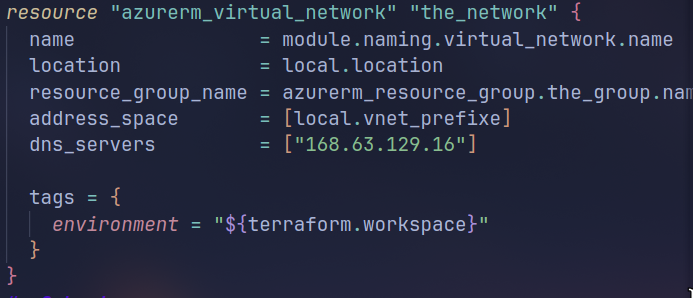
\includegraphics[width=0.8\textwidth]{DNS_server.png}
    \caption{The DNS configuration}
    \label{fig:dns_configuration}
\end{figure}

\section{Conclusion}
This chapter detailed the successful completion of Sprint 1, focusing on provisioning the cloud infrastructure for our project. We presented a modified architecture that removed the application gateway due to cost considerations. The new architecture leverages Terraform modules for efficient code organization and utilizes workspaces to manage different environments (dev, QA, prod) with appropriate resource configurations.
\par
We encountered a challenge during this sprint related to DNS configuration, where the web application struggled to resolve the database hostname. This issue was resolved by leveraging the Azure Wire Server as the default DNS server within the virtual network configuration.
\par
By successfully provisioning the infrastructure and addressing the DNS resolution challenge, Sprint 1 laid the foundation for future sprints to focus on building and deploying the web application and its functionalities.

\clearpage

\chapter{Continuous Integration and Deployment}

\section*{Introduction}
This chapter delves into the core components that establish a robust CI/CD pipeline for our project. We'll explore the setup process, delve into the selection of a branching strategy, and dissect the configuration of pipelines designed for development, staging, and production environments. Each stage within these pipelines will be meticulously explained, highlighting its function and contribution to the overall workflow.
\section{Sprint backlog}
\begin{longtable}[c]{
    |p{.85\textwidth}|
    p{.11\textwidth}|
    }
    \hline
    research the different branching strategies and pick the appropriate one for this project & (2 points) \\
    \hline
    create the build pipeline and publish the artifacts for each environment & (3 points) \\
    \hline
    create the provisioning pipeline for the development environment & (3 points) \\
    \hline
    set up the management of the state file of the terraform in the pipeline & (2 points) \\
    \hline
    create the release pipelines for the staging and production environments & (3 points) \\
    \hline
    test the pipeline by pushing code to the different branches and checking the results & (2 points) \\
    \hline
\end{longtable}
\section{Activities Completed}
\begin{itemize}
    \item \textbf{Azure DevOps account setup:} We created an Azure DevOps account to manage our CI/CD pipeline.
    \item \textbf{picking the right git branching strategy:} We chose the appropriate branching strategy to manage our codebase.
    \item \textbf{creation of the build pipeline:} We created a build pipeline that builds the dotnet core application and publishes the artifacts.
    \item \textbf{creation of the release pipelines:} We created the release pipelines that deploy the artifacts to the different environments depending on the branch.
    \item \textbf{testing the pipeline:} We tested the pipeline by pushing code to the different branches and checking the results.
\end{itemize}

\section{Version Control strategy}
\subsection*{the different branching strategies\cite{webArticle3}:}
\textbf{trunc based development:} In this strategy, requires no branches but instead, developers integrate their changes into a shared trunk at least once a day. This shared trunk should be ready for release anytime.
\begin{itemize}
    \item \textbf{Advantages:} Have better visibility over what changes other developers are making as commits are made directly into the trunk without the need for branches.
    \item \textbf{Desadvantages:} It can be difficult to monitor the quality of the codebase as there are no branches to isolate changes. This approach can be daunting for junior developers as they are interacting directly with the shared trunk.
\end{itemize}
\par
\textbf{github flow:} In this strategy, there is only one branch called the main branch. Developers create feature branches from the main branch, work on their features, and then create a pull request to merge their changes back into the main branch.
\begin{itemize}
    \item \textbf{Advantages:} This strategy is particularly suited for small teams and web applications and it is ideal when you need to maintain a single production version.
    \item \textbf{Desadvantages:} The lack of development branches makes this strategy more susceptible to bugs and so can lead to an unstable production code if branches are not properly tested before merging with the master-release preparation and bug fixes happen in this branch.
\end{itemize}
\par
\textbf{gitflow:} In this strategy, there are two main branches: the master branch and the develop branch. The master branch contains the production-ready code while the develop branch contains the latest code that is ready for release.
\begin{itemize}
    \item \textbf{Advantages:} Perhaps the most obvious benefit of this model is that it allows for parallel development to protect the production code so the main branch remains stable for release while developers work on separate branches.
    \item \textbf{Desadvantages:} Due to GitFlow's complexity, it could slow down the development process and release cycle. In that sense, GitFlow is not an efficient approach for teams wanting to implement continuous integration and continuous delivery.
\end{itemize}
\textbf{gitlab flow:} is a simpler alternative to GitFlow that combines feature-driven development and feature branching with issue tracking. GitLab Flow is great when you want to maintain multiple environments and when you prefer to have a staging environment separate from the production environment.
\begin{itemize}
    \item \textbf{Advantages:} It promotes teamwork and emphasizes code quality with a lean approach, encouraging practices like unit testing and CI/CD.
    \item \textbf{Desadvantages:} With more frequent integration, there's a higher chance of merge conflicts, especially in larger teams.
\end{itemize}
\begin{longtable}[c]{
    |p{.50\textwidth}
    |p{.10\textwidth}|
    p{.30\textwidth}|
    }
    \caption*{the different situations where each branching strategy is suitable}
    \label{tab:gitStratagyTable}
    \\ \hline

    Product type and its release method                                                                                            & Team size & Applicable branching strategy                \\ \hline
    All                                                                                                                            & Small     & Trunk based development                      \\ \hline
    Products that support continuous deployment and release, such as SaaS products                                                 & Middle    & GitHub-Flow and TBD                          \\ \hline
    Products with a definite release window and a periodic version release cadence, such as iOS apps                               & Middle    & Git-Flow and GitLab-Flow with release branch \\ \hline
    Products that are demanding for product quality and support continuous deployment and release, such as basic platform products & Middle    & GitLab-Flow                                  \\ \hline
    Products that are demanding product quality and have a long maintenance cycle for released versions                            & Large     & Git-Flow                                     \\ \hline
\end{longtable}
\par
\textbf{Verdict:} Considering the table's comparison and the advantages and disadvantages listed, GitLab Flow emerges as the optimal choice for our project's workflow since we can leverage its strengths to establish a smooth, efficient, and quality-focused development process for our continuous deployment pipeline.
\subsection*{description of the GitLab flow strategy:}
the GitLab flow strategy consists of 3 main branches: the main branch(develop), the staging branch(pre-prod), and the production branch(prod).

\begin{figure}[htbp]
    \centering
    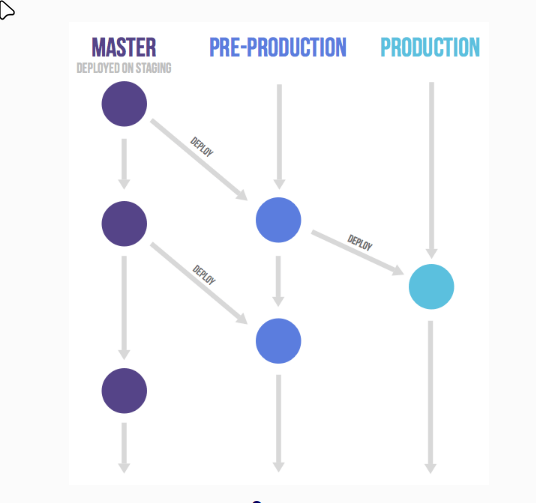
\includegraphics[width=0.6\textwidth]{gitLab.png}
    \caption{gitlab flow strategy}
    \label{fig:gitlab}
\end{figure}

\subsection*{Main branches:}
\begin{itemize}
    \item \textbf{the main branch(develop):} This branch is the default branch and contains the latest code that is ready for release. Developers create feature branches from the main branch, work on their features, and then create a pull request to merge their changes back into the main branch.
    \item \textbf{the staging branch(pre-prod):} This branch is used for testing the code by the QA team before it is deployed to the production environment. The staging branch is created from the main branch and is used to test the code in a production-like environment.
    \item \textbf{the production branch(prod):} This branch contains the production-ready code that is deployed to the production environment. The production branch is created from the staging branch and is used to deploy the code to the production environment.
\end{itemize}
\subsection*{secondary branches:}
these branches are short-lived and are used to develop new features or fix bugs.
\begin{itemize}
    \item \textbf{feature branches:} These branches are created from the main branch and are used to develop new features. Once the feature is complete, a pull request is created to merge the changes back into the main branch.
    \item \textbf{Hotfix branches:} These branches are created from the production branch and are used to fix critical bugs in the production code. Once the bug is fixed, a pull request is created to merge the changes back into the production branch.
\end{itemize}

\section{The CI/CD pipelines}

\subsection*{the build pipeline:}
here's a detailed breakdown of the build pipeline for the .NET Core application:
\begin{itemize}
    \item \textbf{Fetch the code:} The pipeline starts by fetching the latest code from your GitHub repository or a pull request. This is done using a service connection that links our Azure DevOps account to the GitHub repository.
    \item \textbf{Build the code:} This stage involves two main tasks:
          \begin{itemize}
              \item \textbf{Restore dependencies:} The pipeline installs NuGet and restores the packages required for the project. Nuget is the package manager responsible for managing the various dependencies of this application.
              \item \textbf{Build the project:} The pipeline builds the .NET Core project using the dotnet build command.
          \end{itemize}
    \item \textbf{Run tests:} This stage involves running the unit tests and the integration tests to ensure the application functions as expected.
    \item \textbf{Publish artifacts:} The pipeline publishes the build artifacts to the Azure DevOps server. These artifacts are to be used by the release pipeline to deploy the application to the different environments.
\end{itemize}
\subsection*{the release pipeline:}
the release pipeline is the combination of the provisioning and deployment process. Here's a detailed breakdown of the different pipelines for the different environments:
\subsubsection*{the development environment:}
the dev environment is used for testing the code by the developers when a push request is made into the main branch and approval from another developer is required. it consists of the following stages:
\begin{itemize}
    \item \textbf{Fetch the artifacts:} The pipeline starts by fetching the latest artifact that contains the build of the application and the artifact that contains the terraform source code.
    \item \textbf{Deploy the infrastructure:} The pipeline deploys the infrastructure using the terraform source code using the service connection to the Azure subscription.
    \item \textbf{assign the variables:} The pipeline assigns the variables required for the deployment of the application like the name of the web app that is generated during deployment.
    \item \textbf{deploy the application:} The pipeline deploys the application to the web app using the artifact that contains the build of the application.
    \item \textbf{the approval stage:} After the pipeline notifies the responsible developer it waits for his approval to merge the code into the main branch after he is done reviewing the changes using the deployed application.
    \item \textbf{the destruction of the infrastructure:} This stage is used to destroy the infrastructure after the request has been approved or rejected.
\end{itemize}

\begin{figure}[htbp]
    \centering
    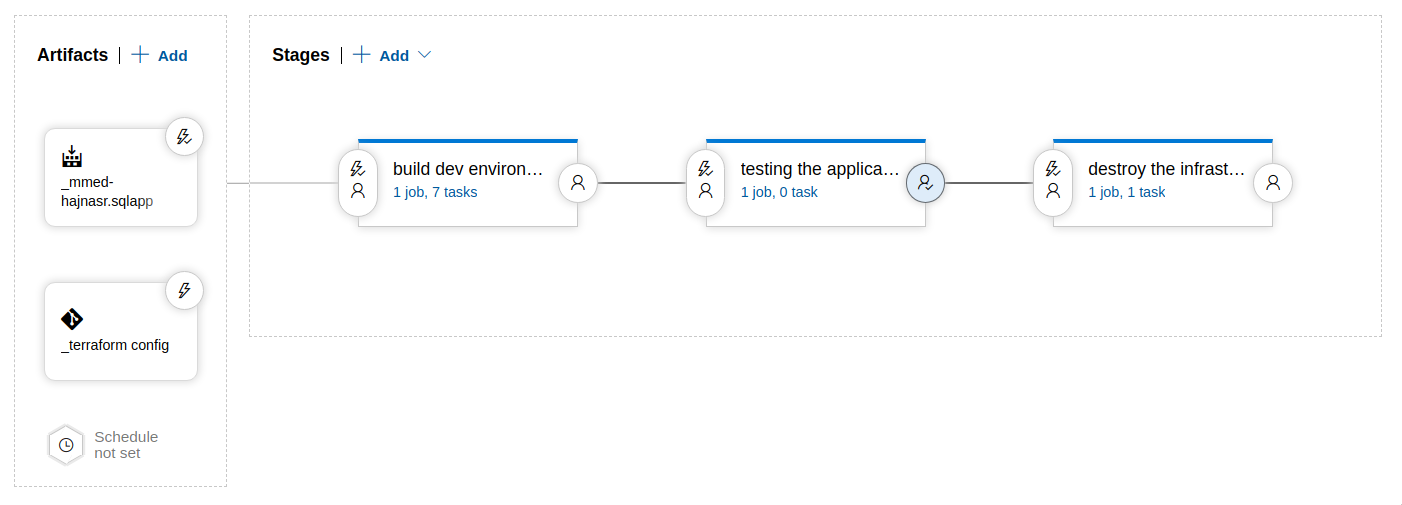
\includegraphics[width=0.9\textwidth]{dev_pipeline.png}
    \caption{development pipeline}
    \label{fig:devPipeline}
\end{figure}

\textbf{the benefits of this pipeline are:}
\begin{itemize}
    \item \textbf{fast feedback:} The pipeline provides fast feedback to the developers on the quality of the code.
    \item \textbf{cost savings:} The pipeline saves costs by destroying the infrastructure after the request has been approved or rejected. so that the infrastructure doesn't keep running when not needed.
    \item \textbf{multiple deployments:} The pipeline allows for multiple deployments in different infrastructures at once due to the randomly generated names. giving us the ability to test multiple pull requests at once.
\end{itemize}
\subsubsection*{the staging and the deployment pipelines:}
\noindent These pipelines share similar stages but differ in their triggers:
\begin{itemize}
    \item \textbf{Staging Pipeline:} Triggered by a push or merge to the pre-production (pre-prod) branch. This environment mirrors production as closely as possible for testing purposes.
    \item \textbf{Deployment Pipeline:} Triggered by a push or merge to the production (prod) branch. This pipeline deploys the application to the live environment used by end users.
\end{itemize}
\noindent The stages within these pipelines typically involve:
\begin{itemize}
    \item \textbf{Fetch the artifacts:} Similar to the development pipeline, this stage retrieves the latest Terraform configuration files and the recently built application artifact.
    \item \textbf{Deploy the infrastructure:} In the staging and production environments, the infrastructure is already deployed using the terraform files. so we directly deploy the application to the web app.
    \item \textbf{Notify Deployment Status:} Once the deployment is complete, the pipeline automatically notifies the designated manager (or team) about the success or failure of the process.
\end{itemize}
\textbf{the benefits of these pipelines are:}
\begin{itemize}
    \item \textbf{Increased Efficiency:} Automating deployments frees up valuable developer and operations time. They can focus on core activities like building new features, improving code quality, and resolving critical issues.
    \item \textbf{Reduced Risk of Errors:} Manual deployments are prone to human error. Staging and deployment pipelines automate the entire process, minimizing the chance of mistakes that could lead to application downtime or malfunctions.
    \item \textbf{Faster Release Cycles:} By automating the deployment process, teams can push new features and bug fixes to staging and production environments much quicker. This eliminates the time spent on manual tasks and allows for more frequent releases, keeping your software up-to-date and competitive.
\end{itemize}
\section{Challenges Faced}
\subsection*{Problem(Secure Terraform State Management in a Multi-Stage Pipeline):}
A critical hurdle encountered during CI/CD pipeline implementation was handling Terraform state files across stages. These files, generated during infrastructure deployment,  contain crucial details about the deployed infrastructure. Terraform relies on them to determine the current state for subsequent actions and this file was required by Terraform to destroy the infrastructure.
\par The initial solution involved saving the state file in an Azure storage account. However, this necessitated granting pipeline access to the storage, incurring potential costs.
\subsection*{solution:}
Further exploration revealed a more efficient approach: utilizing the Azure CLI to destroy deployed resources. By relying solely on the readily accessible resource group name, the Azure CLI could effectively destroy resources after approval/rejection decisions, eliminating the need for storage access and associated costs.
\section*{Conclusion}
The meticulously crafted CI/CD pipeline significantly enhances the development process by automating deployments and infrastructure management. This automation not only minimizes manual work and the potential for errors but also facilitates faster deployments and cost savings through efficient infrastructure utilization.
Our selection of the GitLab Flow branching strategy fosters collaboration and ensures code quality throughout the development lifecycle.
\par
In conclusion, our new CI/CD pipeline empowers our team to deliver features and updates with remarkable efficiency while maintaining an unwavering commitment to quality. As we move forward, the next chapter will explore the various deployment strategies available and delve into the process of selecting and implementing the most suitable option for our specific project requirements.
\clearpage

\chapter*{General Conclusion}
\addcontentsline{toc}{chapter}{General Conclusion}
\markboth{General Conclusion}{}

The document outlines a comprehensive plan to transition from a slow and error-prone deployment process to a significantly faster and more reliable one. This is achieved by embracing a DevOps approach that leverages cloud computing, automation, and modern tools and methodologies. The new approach will automate the entire deployment lifecycle, incorporate security best practices, and utilize Scrum for structured project management.
Following this plan, the initial steps have been successfully completed. This includes provisioning the cloud infrastructure with Terraform modules and establishing a CI/CD pipeline that utilizes GitLab Flow for branching.  These initial steps lay the foundation for future sprints to focus on building and deploying the web application within the cloud environment.
The document concludes by outlining the chosen deployment strategy (blue-green deployment) and the implemented rollback strategy to ensure smooth recovery in case of any issues. Additionally, a monitoring strategy has been established to monitor the health, performance, and usage of the deployed web application. By implementing these comprehensive strategies, the project aims to achieve faster, more reliable deployments with minimal downtime and improved rollback capabilities.
\clearpage

% @author: Stoufa
% the command `\nocite{*}` is mandatory to avoid the “no \citation commands” error
% https://tex.stackexchange.com/questions/18045/problem-with-compiling-bibtex-no-citation-commands-error
%\nocite{*}
\printbibliography[heading=bibintoc]

\chapter*{Annexes}
\addcontentsline{toc}{chapter}{Annexes}
\markboth{Annexes}{}
\stepcounter{chapter}
\addtocontents{lot}{\vspace{3.8mm}}
\addtocontents{lof}{\vspace{3.8mm}}

%Mettez vos annexes ici...

%===================== ANNEXE 1 =====================%
\section*{Annexe 1.~Exemple d'annexe}
\addcontentsline{toc}{section}{Annexe 1.~Exemple d'annexe}

Les chapitres doivent présenter l'essentiel du travail. Certaines informations-trop  détaillées  ou constituant un complément d’information pour toute personne qui désire mieux comprendre ou refaire une expérience décrite dans le document- peuvent être mises au niveau des annexes. Les annexes, {\bf placées après la bibliographie}, doivent donc être numérotées avec des titres (Annexe1, Annexe2, etc.).

\addcontentsline{lot}{table}{Annexe 1.1~~~Exemple tableau dans l'annexe}

Le tableau annexe 1.1 présente un exemple d'un tableau dans l'annexe.

{\raggedright \textbf{Tableau annexe 1.1:}~Exemple tableau dans l'annexe}
\begin{longtable}[c]{
    | p{.20\textwidth}
    | p{.50\textwidth} |
}
    \hline
        0 & 0 \\ \hline 
        1 & 1 \\ \hline 
        2 & 2 \\ \hline
        3 & 3 \\ \hline
        4 & 4 \\
    \hline

\end{longtable}

\newpage
%===================== ANNEXE 2 =====================%
\section*{Annexe 2.~Entreprise}
\addcontentsline{toc}{section}{Annexe 2.~Entreprise}

\addcontentsline{lof}{figure}{Annexe 2.1~~~Logo d'entreprise}

La figure annexe 2.1 présente le logo entreprise.
\begin{figure}[htpb]
    \centering
    \frame{
\includegraphics[width=0.45\columnwidth]{logo-adactim.png}}
    {\\\textbf{Figure annexe 2.1:} Logo d'entreprise}
\end{figure}
\clearpage

\backmatter
%===== File containing the back cover of the document =====%
%                                                          %
% Copyright (C) ISI - All Rights Reserved                  %
% Proprietary                                              %
% Written by Med Hossam <med.hossam@gmail.com>, April 2016 %
%                                                          %
% @author: HEDHILI Med Houssemeddine                       %
% @linkedin: http://tn.linkedin.com/in/medhossam           %
%==========================================================%

%== It's advised to not modify the content of this file ===%
% To set your information, go to global_config.tex file    %
%==========================================================%

\thispagestyle{backcover}
\newgeometry{bottom=25mm,left=15mm,top=20mm,right=15mm}

\begin{changemargin}{3mm}{0cm}
    \begin{minipage}[c]{0.96\columnwidth}
        
        \selectlanguage{english}
        {\LARGE\textbf{Abstract}}
        \vskip1mm
            \begingroup
                \large
                \@englishAbstract
            \endgroup
        \vskip1mm
        {\textbf{Keywords : }
            \begingroup
                \@englishAbstractKeywords
            \endgroup
        }
    \end{minipage}
    
\end{changemargin}

\end{document}